% Options for packages loaded elsewhere
\PassOptionsToPackage{unicode}{hyperref}
\PassOptionsToPackage{hyphens}{url}
\PassOptionsToPackage{dvipsnames,svgnames,x11names}{xcolor}
\documentclass[
  12pt,
]{article}
\usepackage{xcolor}
\usepackage[margin=0.75in]{geometry}
\usepackage{amsmath,amssymb}
\setcounter{secnumdepth}{-\maxdimen} % remove section numbering
\usepackage{iftex}
\ifPDFTeX
  \usepackage[T1]{fontenc}
  \usepackage[utf8]{inputenc}
  \usepackage{textcomp} % provide euro and other symbols
\else % if luatex or xetex
  \usepackage{unicode-math} % this also loads fontspec
  \defaultfontfeatures{Scale=MatchLowercase}
  \defaultfontfeatures[\rmfamily]{Ligatures=TeX,Scale=1}
\fi
\usepackage{lmodern}
\ifPDFTeX\else
  % xetex/luatex font selection
\fi
% Use upquote if available, for straight quotes in verbatim environments
\IfFileExists{upquote.sty}{\usepackage{upquote}}{}
\IfFileExists{microtype.sty}{% use microtype if available
  \usepackage[]{microtype}
  \UseMicrotypeSet[protrusion]{basicmath} % disable protrusion for tt fonts
}{}
\makeatletter
\@ifundefined{KOMAClassName}{% if non-KOMA class
  \IfFileExists{parskip.sty}{%
    \usepackage{parskip}
  }{% else
    \setlength{\parindent}{0pt}
    \setlength{\parskip}{6pt plus 2pt minus 1pt}}
}{% if KOMA class
  \KOMAoptions{parskip=half}}
\makeatother
\usepackage{color}
\usepackage{fancyvrb}
\newcommand{\VerbBar}{|}
\newcommand{\VERB}{\Verb[commandchars=\\\{\}]}
\DefineVerbatimEnvironment{Highlighting}{Verbatim}{commandchars=\\\{\}}
% Add ',fontsize=\small' for more characters per line
\usepackage{framed}
\definecolor{shadecolor}{RGB}{248,248,248}
\newenvironment{Shaded}{\begin{snugshade}}{\end{snugshade}}
\newcommand{\AlertTok}[1]{\textcolor[rgb]{0.94,0.16,0.16}{#1}}
\newcommand{\AnnotationTok}[1]{\textcolor[rgb]{0.56,0.35,0.01}{\textbf{\textit{#1}}}}
\newcommand{\AttributeTok}[1]{\textcolor[rgb]{0.13,0.29,0.53}{#1}}
\newcommand{\BaseNTok}[1]{\textcolor[rgb]{0.00,0.00,0.81}{#1}}
\newcommand{\BuiltInTok}[1]{#1}
\newcommand{\CharTok}[1]{\textcolor[rgb]{0.31,0.60,0.02}{#1}}
\newcommand{\CommentTok}[1]{\textcolor[rgb]{0.56,0.35,0.01}{\textit{#1}}}
\newcommand{\CommentVarTok}[1]{\textcolor[rgb]{0.56,0.35,0.01}{\textbf{\textit{#1}}}}
\newcommand{\ConstantTok}[1]{\textcolor[rgb]{0.56,0.35,0.01}{#1}}
\newcommand{\ControlFlowTok}[1]{\textcolor[rgb]{0.13,0.29,0.53}{\textbf{#1}}}
\newcommand{\DataTypeTok}[1]{\textcolor[rgb]{0.13,0.29,0.53}{#1}}
\newcommand{\DecValTok}[1]{\textcolor[rgb]{0.00,0.00,0.81}{#1}}
\newcommand{\DocumentationTok}[1]{\textcolor[rgb]{0.56,0.35,0.01}{\textbf{\textit{#1}}}}
\newcommand{\ErrorTok}[1]{\textcolor[rgb]{0.64,0.00,0.00}{\textbf{#1}}}
\newcommand{\ExtensionTok}[1]{#1}
\newcommand{\FloatTok}[1]{\textcolor[rgb]{0.00,0.00,0.81}{#1}}
\newcommand{\FunctionTok}[1]{\textcolor[rgb]{0.13,0.29,0.53}{\textbf{#1}}}
\newcommand{\ImportTok}[1]{#1}
\newcommand{\InformationTok}[1]{\textcolor[rgb]{0.56,0.35,0.01}{\textbf{\textit{#1}}}}
\newcommand{\KeywordTok}[1]{\textcolor[rgb]{0.13,0.29,0.53}{\textbf{#1}}}
\newcommand{\NormalTok}[1]{#1}
\newcommand{\OperatorTok}[1]{\textcolor[rgb]{0.81,0.36,0.00}{\textbf{#1}}}
\newcommand{\OtherTok}[1]{\textcolor[rgb]{0.56,0.35,0.01}{#1}}
\newcommand{\PreprocessorTok}[1]{\textcolor[rgb]{0.56,0.35,0.01}{\textit{#1}}}
\newcommand{\RegionMarkerTok}[1]{#1}
\newcommand{\SpecialCharTok}[1]{\textcolor[rgb]{0.81,0.36,0.00}{\textbf{#1}}}
\newcommand{\SpecialStringTok}[1]{\textcolor[rgb]{0.31,0.60,0.02}{#1}}
\newcommand{\StringTok}[1]{\textcolor[rgb]{0.31,0.60,0.02}{#1}}
\newcommand{\VariableTok}[1]{\textcolor[rgb]{0.00,0.00,0.00}{#1}}
\newcommand{\VerbatimStringTok}[1]{\textcolor[rgb]{0.31,0.60,0.02}{#1}}
\newcommand{\WarningTok}[1]{\textcolor[rgb]{0.56,0.35,0.01}{\textbf{\textit{#1}}}}
\usepackage{longtable,booktabs,array}
\usepackage{calc} % for calculating minipage widths
% Correct order of tables after \paragraph or \subparagraph
\usepackage{etoolbox}
\makeatletter
\patchcmd\longtable{\par}{\if@noskipsec\mbox{}\fi\par}{}{}
\makeatother
% Allow footnotes in longtable head/foot
\IfFileExists{footnotehyper.sty}{\usepackage{footnotehyper}}{\usepackage{footnote}}
\makesavenoteenv{longtable}
\usepackage{graphicx}
\makeatletter
\newsavebox\pandoc@box
\newcommand*\pandocbounded[1]{% scales image to fit in text height/width
  \sbox\pandoc@box{#1}%
  \Gscale@div\@tempa{\textheight}{\dimexpr\ht\pandoc@box+\dp\pandoc@box\relax}%
  \Gscale@div\@tempb{\linewidth}{\wd\pandoc@box}%
  \ifdim\@tempb\p@<\@tempa\p@\let\@tempa\@tempb\fi% select the smaller of both
  \ifdim\@tempa\p@<\p@\scalebox{\@tempa}{\usebox\pandoc@box}%
  \else\usebox{\pandoc@box}%
  \fi%
}
% Set default figure placement to htbp
\def\fps@figure{htbp}
\makeatother
\setlength{\emergencystretch}{3em} % prevent overfull lines
\providecommand{\tightlist}{%
  \setlength{\itemsep}{0pt}\setlength{\parskip}{0pt}}
\usepackage{fancyhdr}
\pagestyle{fancy}
\fancyfoot{}
\usepackage[default]{sourcesanspro}
\usepackage{parskip}
\usepackage{geometry}
\usepackage{caption}
\usepackage{xcolor}
\definecolor{green}{RGB}{0,102,0}
\definecolor{blue}{RGB}{0, 0, 139}
\definecolor{darkcerulean}{rgb}{0.03, 0.27, 0.49}
\definecolor{darkmidnightblue}{rgb}{0.0, 0.2, 0.4}
\AtBeginDocument{\let\maketitle\relax}
\usepackage[none]{hyphenat}
\usepackage[document]{ragged2e}
\usepackage{graphicx}
\usepackage{geometry}
\usepackage{sectsty}\allsectionsfont{\raggedright}
\usepackage{sectsty}\sectionfont{\centering\color{darkmidnightblue}}
\usepackage{sectsty}\subsectionfont{\centering\color{darkmidnightblue}}
\usepackage{titlesec}
\usepackage{longtable}
\usepackage{tabu}
\usepackage{wrapfig}
\usepackage[export]{adjustbox}
\titlespacing{\section}{0pt}{24pt plus 2pt minus 1pt}{0pt plus 1pt minus 1pt}
\titlespacing{\subsection}{0pt}{12pt plus 2pt minus 1pt}{0pt plus 1pt minus 1pt}
\titlespacing{\subsubsection}{0pt}{12pt plus 2pt minus 1pt}{0pt plus 1pt minus 1pt}
\usepackage{pdflscape}
\newcommand{\blandscape}{\begin{landscape}}
\newcommand{\elandscape}{\end{landscape}}
\usepackage{floatrow}
\DeclareFloatSeparators{mysep}{\hskip-94em}
\floatsetup[figure]{capposition=beside,capbesidesep=mysep,capbesideposition={right, center}}
\usepackage{booktabs}
\usepackage{longtable}
\usepackage{array}
\usepackage{multirow}
\usepackage{wrapfig}
\usepackage{float}
\usepackage{colortbl}
\usepackage{pdflscape}
\usepackage{tabu}
\usepackage{threeparttable}
\usepackage{threeparttablex}
\usepackage[normalem]{ulem}
\usepackage{makecell}
\usepackage{xcolor}
\usepackage{bookmark}
\IfFileExists{xurl.sty}{\usepackage{xurl}}{} % add URL line breaks if available
\urlstyle{same}
\hypersetup{
  pdftitle={Syllabus},
  pdfauthor={Emilio M. Bruna},
  colorlinks=true,
  linkcolor={blue},
  filecolor={Maroon},
  citecolor={Blue},
  urlcolor={blue},
  pdfcreator={LaTeX via pandoc}}

\title{Syllabus}
\author{Emilio M. Bruna}
\date{2025}

\begin{document}
\maketitle

\thispagestyle{empty}

\begin{center}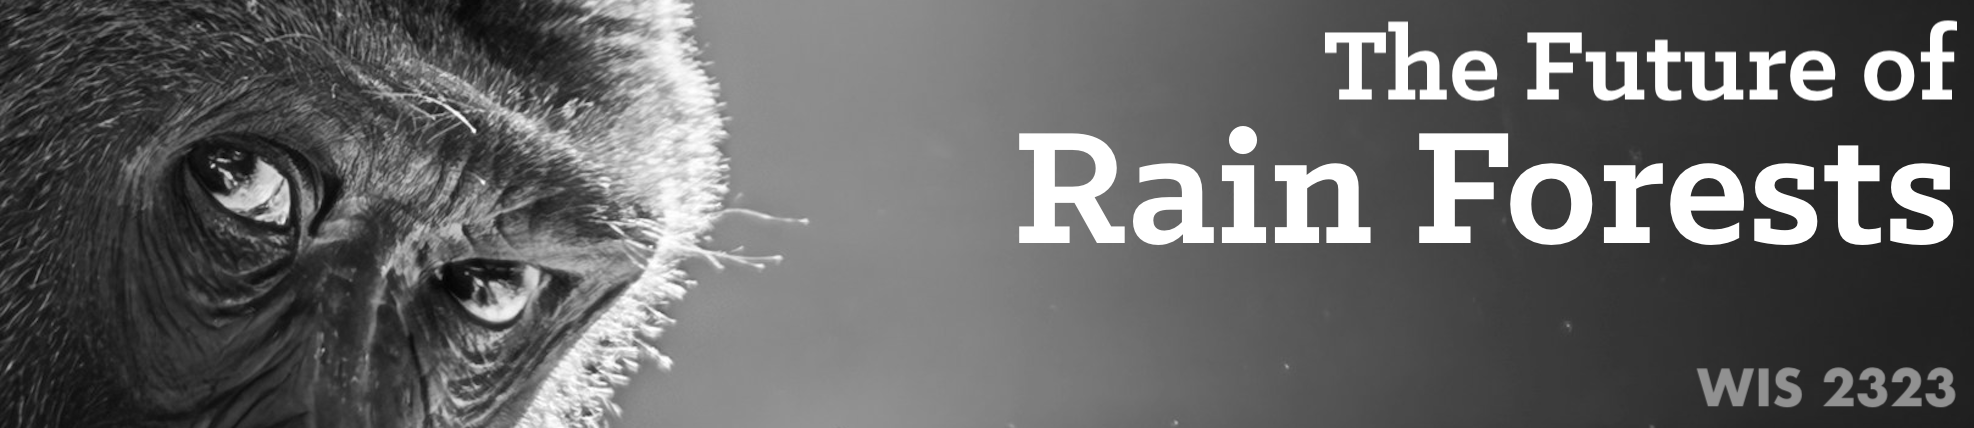
\includegraphics[width=1\linewidth]{./icons/banner} \end{center}

\begin{longtable}[]{@{}
  >{\raggedright\arraybackslash}p{(\linewidth - 8\tabcolsep) * \real{0.2000}}
  >{\raggedright\arraybackslash}p{(\linewidth - 8\tabcolsep) * \real{0.2000}}
  >{\raggedright\arraybackslash}p{(\linewidth - 8\tabcolsep) * \real{0.2000}}
  >{\raggedright\arraybackslash}p{(\linewidth - 8\tabcolsep) * \real{0.2000}}
  >{\raggedright\arraybackslash}p{(\linewidth - 8\tabcolsep) * \real{0.2000}}@{}}
\toprule\noalign{}
\begin{minipage}[b]{\linewidth}\raggedright
\end{minipage} & \begin{minipage}[b]{\linewidth}\raggedright
Instructor
\end{minipage} & \begin{minipage}[b]{\linewidth}\raggedright
TA
\end{minipage} & \begin{minipage}[b]{\linewidth}\raggedright
Class Sessions
\end{minipage} & \begin{minipage}[b]{\linewidth}\raggedright
Location
\end{minipage} \\
\midrule\noalign{}
\endhead
\bottomrule\noalign{}
\endlastfoot
\pandocbounded{
\includegraphics[keepaspectratio]{./icons/hummingbird.png}}
& Dr.~Emilio M. Bruna
\href{mailto:embruna@ufl.edu}{\nolinkurl{embruna@ufl.edu}} 352.846.0634
& Priyanka Hari Haran
\href{mailto:phariharan1@ufl.edu}{\nolinkurl{phariharan1@ufl.edu}}
352.846.0527 & Tuesdays 3:00-3:50 and Thursdays 3:00-4:55 & LIT 0231
(both days) \\
\end{longtable}

\vspace{0.5cm}

\begin{table}[H]
\centering
\begin{tabular}[t]{>{\centering\arraybackslash}m{10em}>{\centering\arraybackslash}m{10em}>{\centering\arraybackslash}m{11em}>{\centering\arraybackslash}m{6em}}

\cellcolor{white}{\textcolor{black}{\textbf{\color{darkmidnightblue}Instructor}}} & \cellcolor{white}{\textcolor{black}{\textbf{\color{darkmidnightblue}Teaching Assistant}}} & \cellcolor{white}{\textcolor{black}{\textbf{\color{darkmidnightblue}Class Sessions}}} & \cellcolor{white}{\textcolor{black}{\textbf{\color{darkmidnightblue}Location}}}\\
\cellcolor{white}{\textcolor{black}{Dr. Emilio M. Bruna}} & \cellcolor{white}{\textcolor{black}{Priyanka Hari Haran}} & \cellcolor{white}{\textcolor{black}{Tuesdays 3:00-3:50 and}} & \cellcolor{white}{\textcolor{black}{LIT 0231}}\\
\cellcolor{white}{\textcolor{black}{embruna@ufl.edu}} & \cellcolor{white}{\textcolor{black}{phariharan1@ufl.edu}} & \cellcolor{white}{\textcolor{black}{Thursdays 3:00-4:55}} & \cellcolor{white}{\textcolor{black}{(both days)}}\\
\cellcolor{white}{\textcolor{black}{352.846.0634}} & \cellcolor{white}{\textcolor{black}{352.846.0527}} & \cellcolor{white}{\textcolor{black}{}} & \cellcolor{white}{\textcolor{black}{}}\\
\end{tabular}
\end{table}

\vspace{-0.5cm}

This course investigates the fundamental issues addressed by scientists
studying tropical rain forests, including what gave rise to their
remarkable biodiversity, the drivers and consequences of deforestation,
why people are fascinated by rain forests, cultural stereotypes about
the tropics, and if forest conservation is compatible with socioeconomic
development. \textbf{\emph{By the end of the course students will be
able to:}}

\begin{itemize}
\tightlist
\item
  Recognize and describe stereotypes about rain forests \& their
  residents
\item
  Analyze rain forest tropes in art, literature, \& popular culture
\item
  Discuss \& evaluate hypotheses for the origins and maintenance of
  tropical biodiversity
\item
  Explain \& compare human history in rain forests
\item
  Review contemporary threats to rain forests
\item
  Analyze and visualize data on deforestation
\item
  Review and contrast strategies for rain forest conservation \&
  restoration
\item
  Identify rain forests in their daily lives \& set personal goals for
  advancing their conservation
\item
  Produce materials for communicating about rain forests to family and
  peers
\end{itemize}

\vspace{0.3cm}

\begin{figure}


\includegraphics[width=0.03\linewidth]{./icons/hummingbird} \hfill{}

\caption{GenEd and Quest Information}\label{fig:gened_details}
\end{figure}

\vspace{-0.3cm}

\textbf{A minimum grade of C is required for Quest and General Education
credit.} Courses intended to satisfy Quest and General Education
requirements cannot be taken S-U. \emph{This course fulfills the
following Quest and GenEd requirements:}

\begin{itemize}
\tightlist
\item
  Quest 2
\item
  GenEd International
\item
  \emph{Credits:} 3
\item
  \emph{Prerequisites:} None
\end{itemize}

\vspace{0.2cm}

\textbf{This also counts towards a minor or certificate in Latin
American Studies.}\\
See
\href{https://www.latam.ufl.edu/academics/undergraduate-programs/}{www.latam.ufl.edu/academics/undergraduate-programs}
for more information.

\begin{figure}


\includegraphics[width=0.03\linewidth]{./icons/gorilla} \hfill{}

\caption{Required Course Materials   }\label{fig:materials}
\end{figure}

\vspace{-0.3cm}

\textbf{Students are not required to purchase any textbooks or course
materials;} all materials, including readings and videos, will be
available on the course Canvas page. However, many of the assigned
readings from the \emph{New York Times} and \emph{Washington Post} have
dynamic multimedia data visualizations and video that can't be
appreciated in the posted .pdf format. \emph{Students in this class
should sign up for free online access to the New York Times} and
\emph{Washington Post} by following the instructions at
\href{https://businesslibrary.uflib.ufl.edu/c.php?g=943928&p=7708734}{this
UF Libraries Website}.

\textbf{Materials and Supplies Fees}: None.

\newpage

\begin{figure}[h]


\includegraphics[width=0.03\linewidth]{./icons/beetle} \hfill{}

\caption{Instructor and TA Office Hours}\label{fig:office_hours}
\end{figure}

\textbf{Instructor:} Wednesday \& Friday 1:30-3:00 pm (in-person \&
online). Drop by anytime or sign up for a specific time here:
\url{https://embruna.youcanbook.me}.

\textbf{Teaching Assistant:} Tuesday 1:00-2:30 pm (in-person \& online).

\begin{itemize}
\item
  \textbf{\emph{Location - in-person:}} The Tropical Ecology \&
  Conservation Lab is located next to the Rawlings Hall bus stop (711
  Newell Drive; to find a map click the ``Contact'' link at
  \href{http://brunalab.org}{BrunaLab.org}).
\item
  \textbf{\emph{Location - online:}} use the zoom link on the course
  Canvas page. We are online the entire session.
\end{itemize}

\textbf{If you can't make it these days/times:} Please let us know - we
will find a time to meet that works for you.

\begin{center}\rule{0.5\linewidth}{0.5pt}\end{center}

\vspace{-0.7cm}

\begin{Shaded}
\begin{Highlighting}[]
\NormalTok{knitr}\SpecialCharTok{::}\FunctionTok{include\_graphics}\NormalTok{(}\StringTok{"./icons/vine.png"}\NormalTok{)}
\end{Highlighting}
\end{Shaded}


\includegraphics[width=0.1\linewidth]{./icons/vine}

\section{Assignments, Grades, \&
Participation}\label{assignments-grades-participation}

\vspace{0.3cm}

Learning in our class is achieved with an diverse array of methods
ranging from data analysis to essays to projects. In most class sessions
you will also be working with small groups of students to complete an
in-class assignment that reinforces the major themes of the day's topic.
In keeping with the philosophy of the Quest program, this course also
has \emph{Experiential Learning and Self-Reflection Components}. For
details on the different types of assignments and the Quest Learning
Components, see course Canvas page.

\vspace{0.1cm}

\begin{figure}


\includegraphics[width=0.03\linewidth]{./icons/vine} \hfill{}

\caption{Assignments (1000 points total)}\label{fig:grading}
\end{figure}

\vspace{-0.5cm}

\begin{center}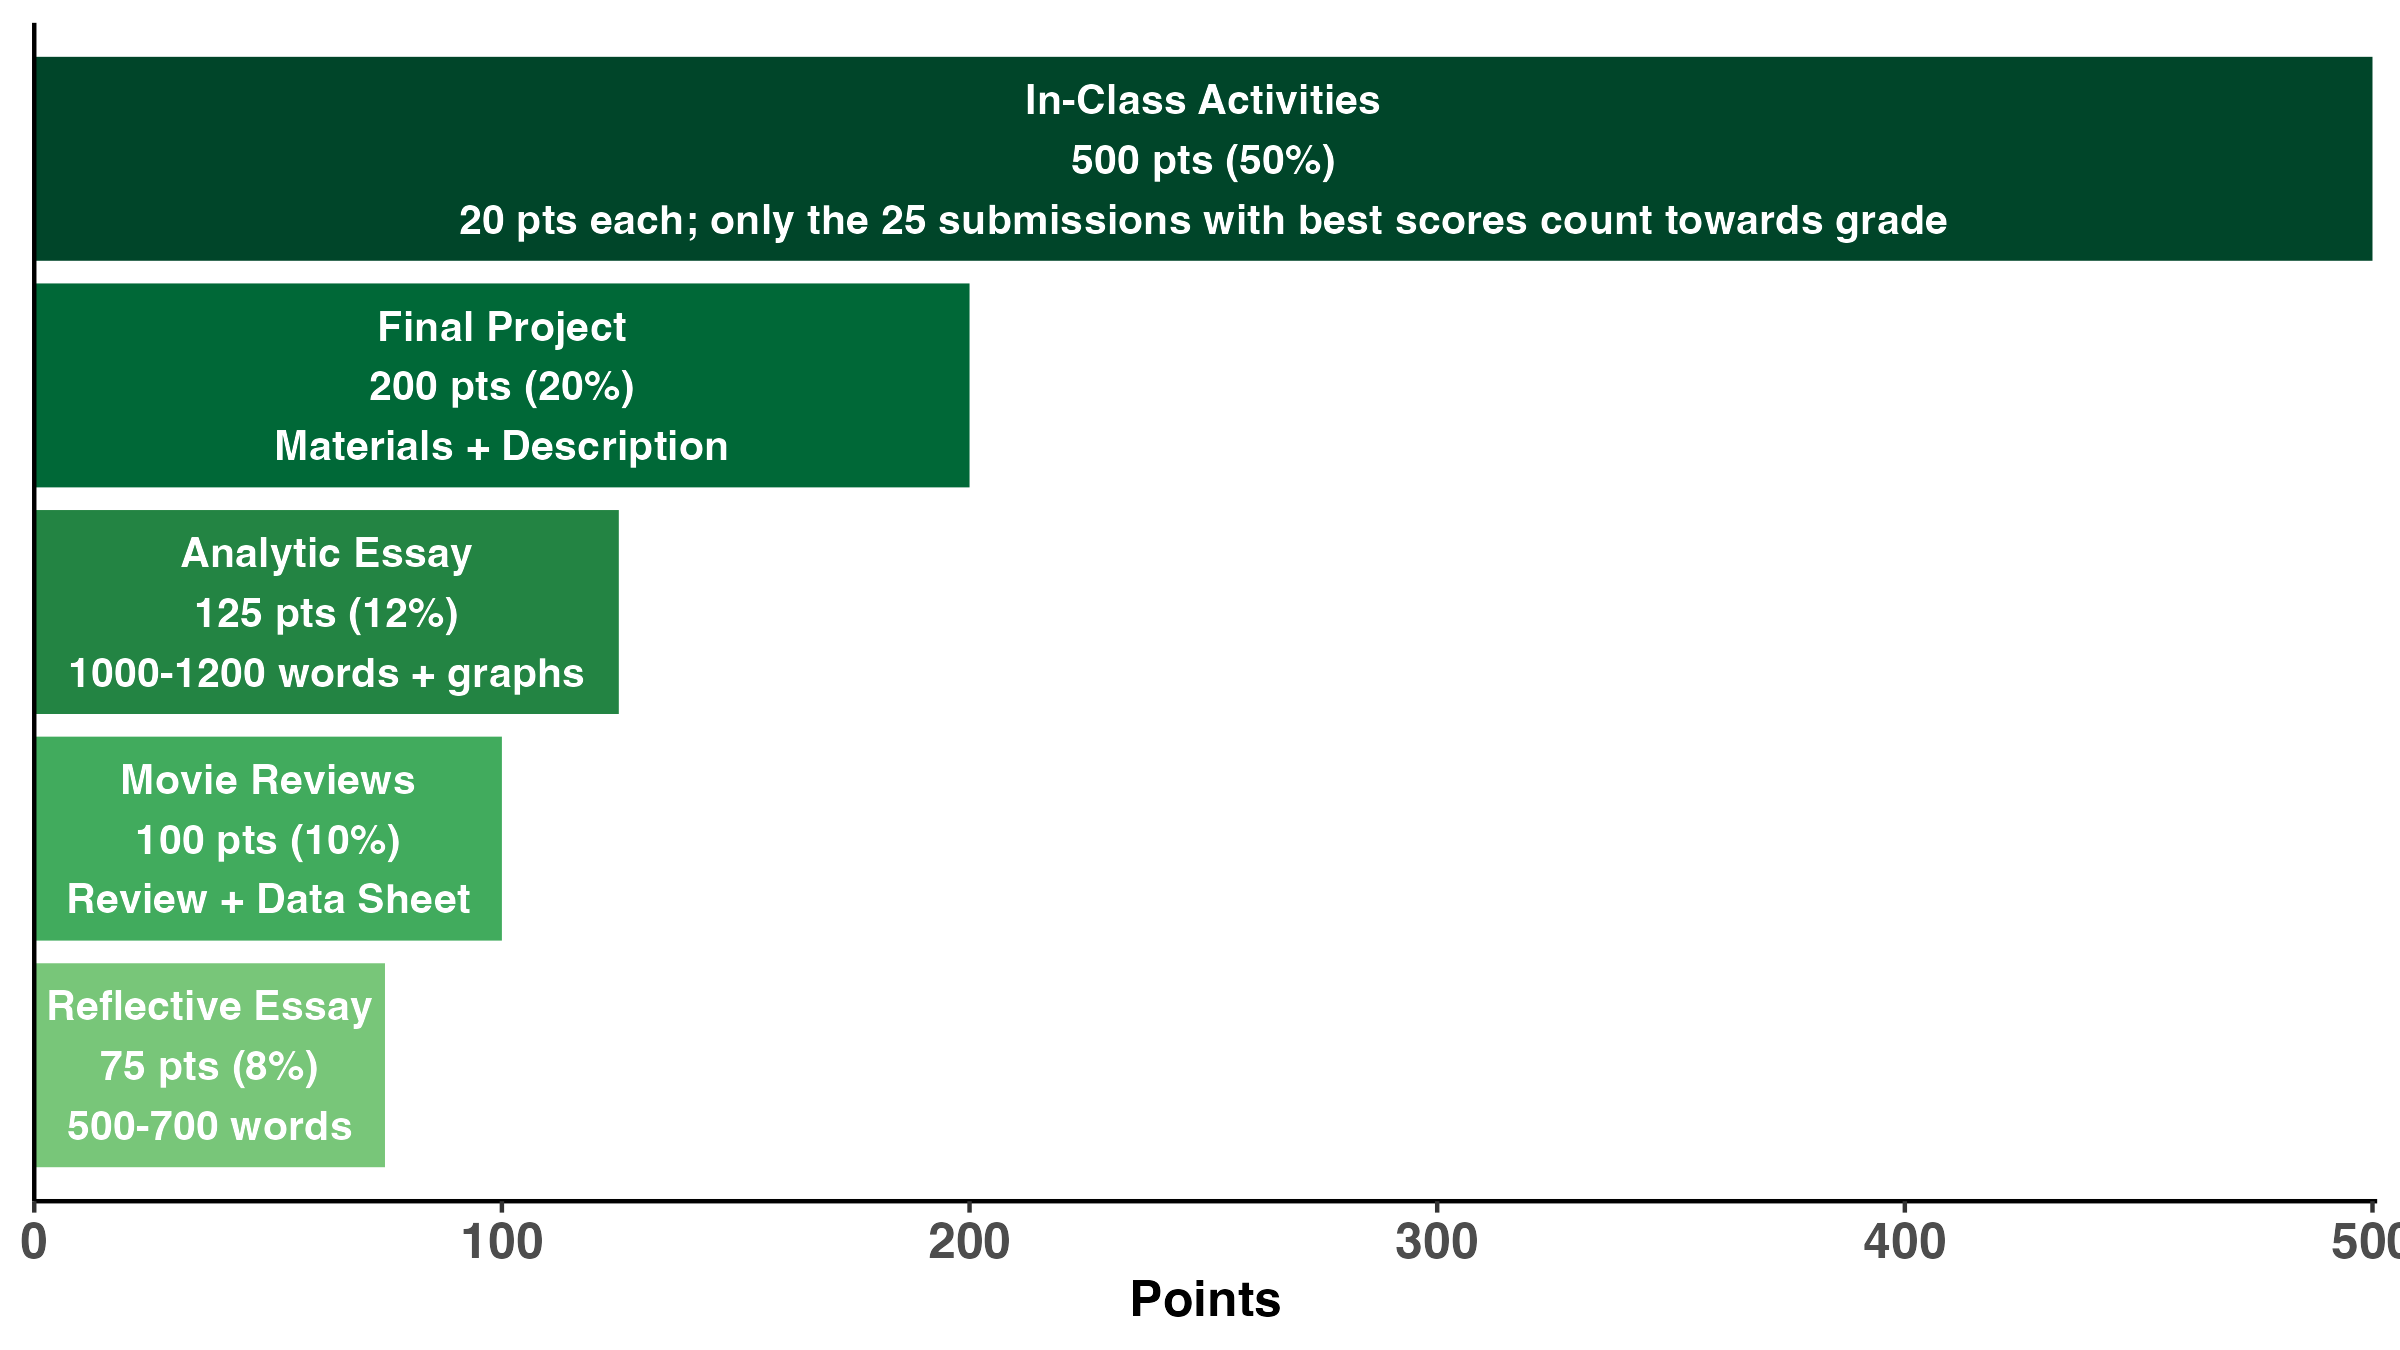
\includegraphics[width=0.85\linewidth]{./icons/hw} \end{center}

\textbf{In-class Assignments are due by the following class session.}
Late assignments will lose 10 pts.

\textbf{\emph{Regrades:}} Requests for re-evaluation of assignments must
be accompanied by an explanation for why you think you deserve
additional credit and the number of additional points you think you
deserve. The deadline for submission is one week after the work was
returned.

\textbf{\emph{Grade Assignment}} (based on \% of total points earned): A
= 94--100\%, A- = 90--93\%, B+ = 87--89\%, B = 84--86\%, B- = 80--83\%,
C+ = 77--79\%, C = 74--76\%, C- = 70--73\%, D+ = 67--69\%, D = 64--66\%,
D- = 60--63\%, E\textless60

\textbf{\emph{Grade Points:}} For information on how UF assigns grade
points, visit:
\newline \textless{}\url{https://catalog.ufl.edu/UGRD/academic-regulations/grades-grading-policies/}

\begin{figure}


\includegraphics[width=0.03\linewidth]{./icons/monkey} \hfill{}

\caption{Attendance and Participation}\label{fig:attendance}
\end{figure}

\vspace{-0.3cm}

\textbf{\emph{Attendance:}} Though attendance is not required, many of
the sessions we will be completing activities in class that count
towards your grade. Most of these can be completed independently, but by
doing them in class you will benefit from working collaboratively with
the other students.

\emph{Some of the in-class activities can not be completed outside of
class time.} If you miss class on one one of these days, that is why the
grade for in-class activities is based on a subset of the total
activities; you can also elect to make up lost points with extra-credit
assignments. \emph{If you need to miss class for any reason, please let
me know as soon as possible}. We will make arrangements for you to
complete any assignments and go over any material you will be missing. I
would much rather you focus on your health, attend your conference, or
support friends and family in need than struggle to turn in assignments.

\textbf{\emph{Participation:}} Consistent informed, thoughtful, and
considerate class participation is encouraged (and in some cases
required). \emph{If you have personal issues that prohibit you from
joining freely in class discussion (e.g., shyness, language barriers,
medical condition): no problem.} let us know and we will discuss
alternative modes of participation.

\textbf{\emph{Important note regarding class discussions and group
work:}} We will explore some challenging, important problems and
increase our understandings of different perspectives and approaches for
addressing them. These conversations may not always be easy; we
sometimes will make mistakes in both how we communicate our perspective
and what we hear other say. There may be times when we need patience,
courage, imagination, and of course mutual respect to engage our texts,
classmates, instructors, guests, and our own ideas and experiences.
\emph{Disrespectful or disruptive behavior will not be tolerated}. And
always remember that as scholars we must employ critical thinking, rely
on data, and cite verifiable sources and experts to interrogate all
assigned readings and subject matter in this course as a means of
determining if we agree with classmates and instructors. No lesson is
intended to espouse, promote, advance, inculcate, or compel a particular
feeling, perception, viewpoint or belief.

\begin{center}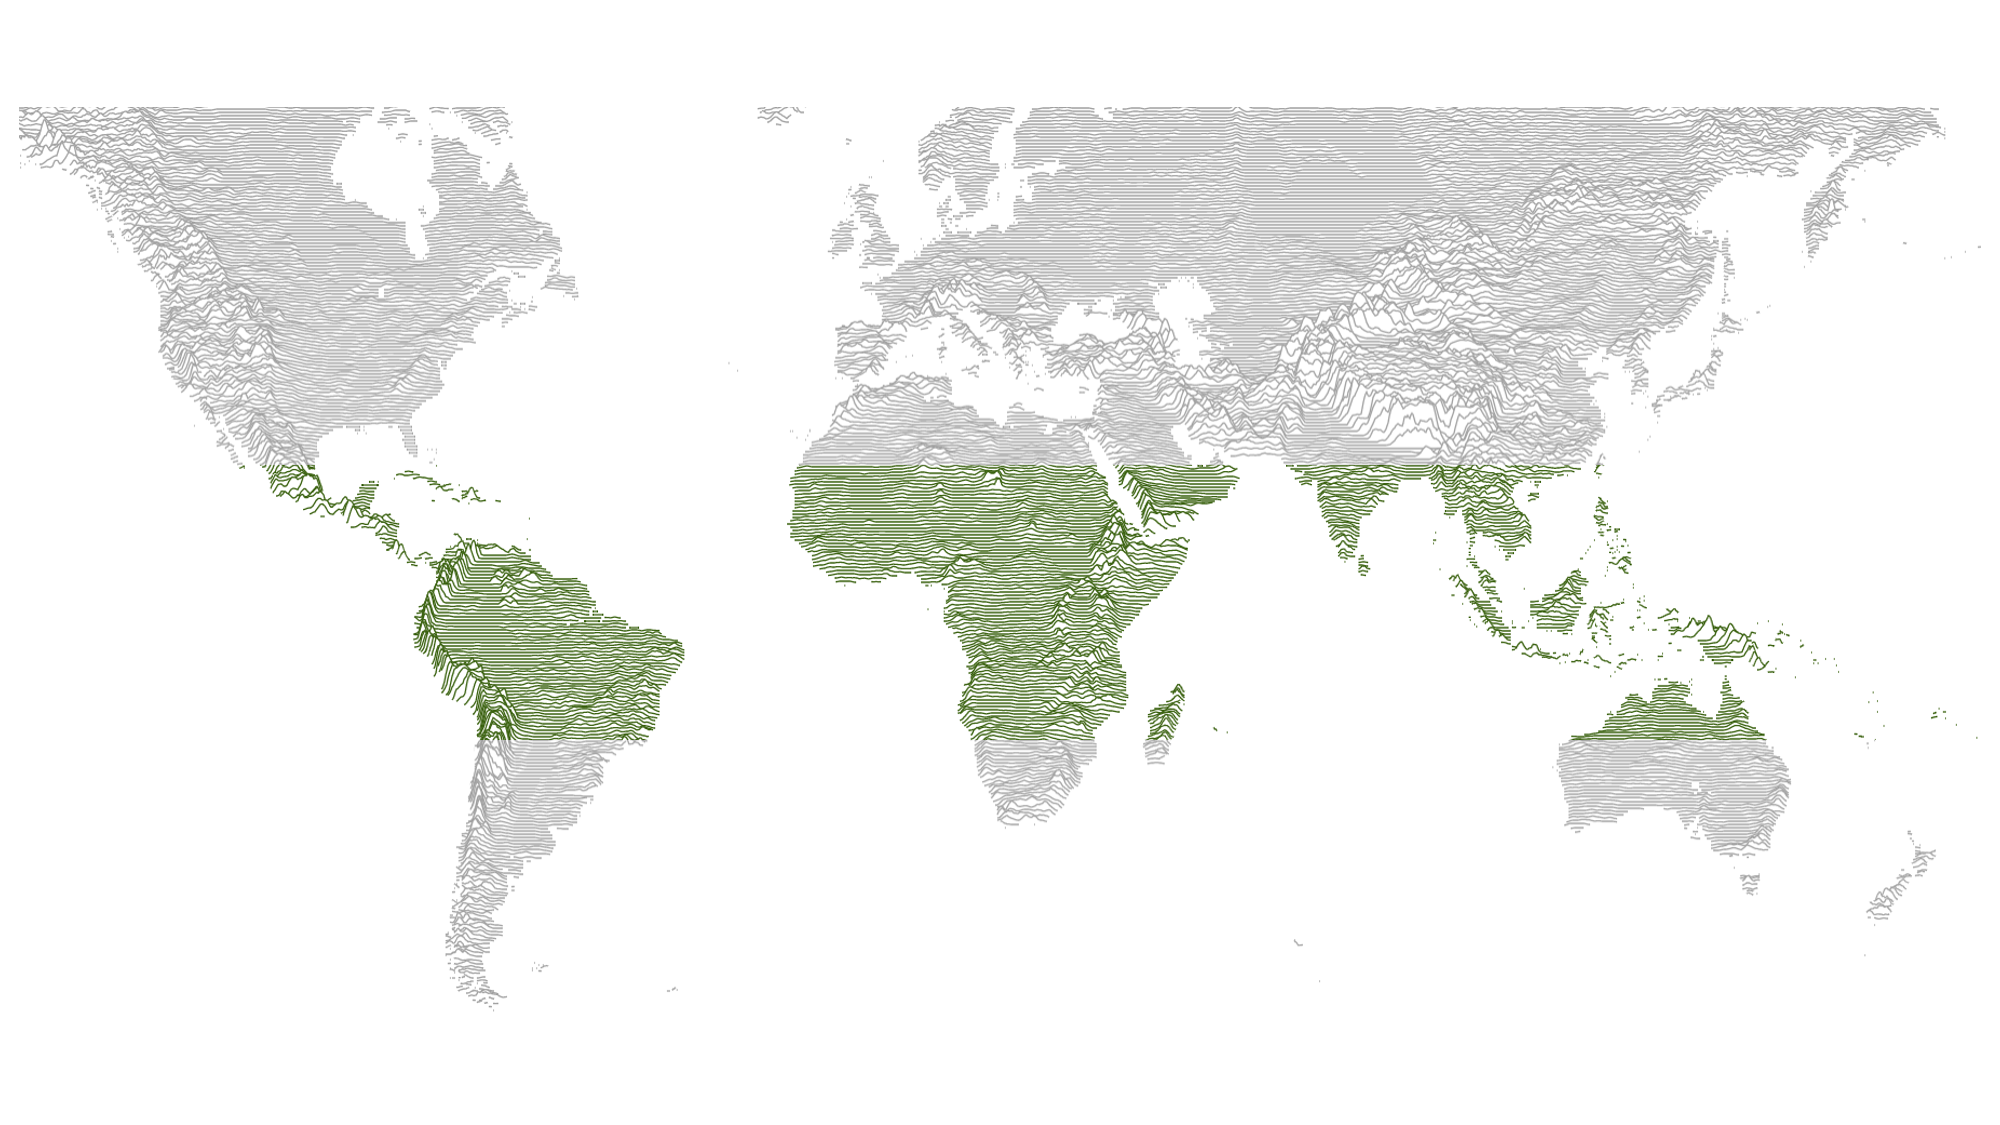
\includegraphics[width=0.9\linewidth]{./icons/ridges} \end{center}

\section{Semester Overview \& Key
Dates}\label{semester-overview-key-dates}

\vspace{0.0cm}

\begin{table}[H]
\centering\begingroup\fontsize{50}{52}\selectfont

\fontsize{10}{12}\selectfont
\resizebox{\ifdim\width>\linewidth\linewidth\else\width\fi}{!}{
\fontsize{8}{10}\selectfont
\begin{tabu} to \linewidth {>{\raggedright\arraybackslash}p{6em}>{\raggedright\arraybackslash}p{1em}>{\raggedright\arraybackslash}p{4em}>{\raggedright\arraybackslash}p{23em}>{}l}
\toprule
\textbf{WEEK} & \textbf{ } & \textbf{DATE} & \textbf{TOPIC} & \textbf{ASSIGNMENT DISTRIBUTED or DUE}\\
\midrule
\addlinespace[0.3em]
\multicolumn{5}{l}{\textbf{WHY ARE WE FASCINATED BY TROPICAL RAIN FORESTS?}}\\
\hspace{1em}Week 1 & 1 & 22-Aug & Class Starts Thursday! & \textbf{}\\
\hspace{1em} & 2 & 21-Aug & Course Welcome and Introduction & \textbf{}\\
\hspace{1em} &  &  &  \vphantom{15} & \textbf{}\\
\hspace{1em}Week 2 & 1 & 26-Aug & Historical Narratives & \textbf{}\\
\hspace{1em} & 2 & 28-Aug & Rain forest imagery in Art \& Lit & \textbf{}\\
\hspace{1em} &  &  &  \vphantom{14} & \textbf{}\\
\hspace{1em}Week 3 & 1 & 2-Sep & The Rain Forest in Pop Culture & \textbf{Movie Reviews Assigned}\\
\addlinespace[0.3em]
\multicolumn{5}{l}{\textbf{THE ECOLOGY \& EVOLUTION OF TROPICAL RAIN FORESTS}}\\
\hspace{1em} & 2 & 4-Sep & What is a Rain Forest? & \textbf{}\\
\hspace{1em} &  &  &  \vphantom{13} & \textbf{}\\
\hspace{1em}Week 4 & 1 & 9-Sep & What else is a Rain Forest? & \textbf{}\\
\hspace{1em} & 2 & 11-Sep & Patterns of Biodiversity 1 & \textbf{}\\
\hspace{1em} &  &  &  \vphantom{12} & \textbf{}\\
\hspace{1em}Week 5 & 1 & 16-Sep & Patterns of Biodiversity 2 & \textbf{}\\
\hspace{1em} & 2 & 18-Sep & Origins of tropical biodiversity & \textbf{}\\
\hspace{1em} &  &  &  \vphantom{11} & \textbf{}\\
\hspace{1em}Week 6 & 1 & 23-Sep & Maintenance of tropical biodiversity - FLMNH Trip & \textbf{}\\
\hspace{1em} & 2 & 25-Sep & The Paradox of Luxuriance \& Forest disturbance & \textbf{}\\
\hspace{1em} &  &  &  \vphantom{10} & \textbf{}\\
\hspace{1em}Week 7 & 1 & 30-Sep & Humans are part of rain forests & \textbf{}\\
\hspace{1em} & 2 & 2-Oct & Narratives Revisited: Biology, History, Fiction, Reality & \textbf{Movie Reviews Due}\\
\hspace{1em} &  &  &  \vphantom{9} & \textbf{}\\
\hspace{1em}Week 8 & 1 & 7-Oct & JUNGLE FILM FESTIVAL (Evening Screening, 7 pm) & \textbf{}\\
\addlinespace[0.3em]
\multicolumn{5}{l}{\textbf{THE DRIVERS AND IMPACTS OF DEFORESTATION}}\\
\hspace{1em} & 2 & 9-Oct & How much Tropical Rain Forest is there? & \textbf{}\\
\hspace{1em} &  &  &  \vphantom{8} & \textbf{}\\
\hspace{1em}Week 9 & 1 & 14-Oct & How much Tropical Rain Forest have we lost? & \textbf{Analytic Essay Assigned}\\
\hspace{1em} & 2 & 16-Oct & Drivers of Deforestation: Timber, Mining, Infrastructure & \textbf{}\\
\hspace{1em} &  &  &  \vphantom{7} & \textbf{}\\
\hspace{1em}Week 10 & 1 & 21-Oct & Drivers of Deforestation: Agriculture & \textbf{}\\
\hspace{1em} & 2 & 23-Oct & Climate change and Tropical Forests & \textbf{}\\
\hspace{1em} &  &  &  \vphantom{6} & \textbf{}\\
\addlinespace[0.3em]
\multicolumn{5}{l}{\textbf{THE FUTURE OF TROPICAL RAIN FORESTS}}\\
\hspace{1em}Week 11 & 1 & 28-Oct & Addressing Climate change & \textbf{Analytic Essay Due}\\
\hspace{1em} & 2 & 30-Oct & Consumer choices & \textbf{Reflective Essay Assigned}\\
\hspace{1em} &  &  &  \vphantom{5} & \textbf{}\\
\hspace{1em}Week 12 & 1 & 4-Nov & DURIAN FEST & \textbf{}\\
\hspace{1em} & 2 & 6-Nov & International frameworks & \textbf{}\\
\hspace{1em} &  &  &  \vphantom{4} & \textbf{}\\
\hspace{1em}Week 13 & 1 & 11-Nov & Local Initiatives, Empowered Communities, \& Activism & \textbf{Reflective Essay Due}\\
\hspace{1em} & 2 & 13-Nov & Protected areas & \textbf{Final Project Assigned}\\
\hspace{1em} &  &  &  \vphantom{3} & \textbf{}\\
\hspace{1em}Week 14 & 1 & 18-Nov & Forest restoration \& regeneration & \textbf{}\\
\hspace{1em} & 2 & 20-Nov & Tropical Rain Forests \& Global Health & \textbf{}\\
\hspace{1em} &  &  &  \vphantom{2} & \textbf{}\\
\hspace{1em}Week 15 & 1 & 25-Nov & No class - Thanksgiving & \textbf{}\\
\hspace{1em} & 2 & 27-Nov & No class - Thanksgiving & \textbf{}\\
\hspace{1em} &  &  &  \vphantom{1} & \textbf{}\\
\hspace{1em}Week 16 & 1 & 2-Dec & Rain Forest Headlines  / What will you do? & \textbf{}\\
\hspace{1em} & 2 & 4-Dec & No Class - Reading Days & \textbf{}\\
\hspace{1em} &  &  &  & \textbf{}\\
\textbf{Finals Week} & \textbf{} & \textbf{9-Dec} & \textbf{Finals Week} & \textbf{\textbf{Final Day to Submit Work}}\\
\bottomrule
\end{tabu}}
\endgroup{}
\end{table}

\end{document}
